\documentclass{beamer}

\title{Image Classification Project}
\author{Your Name}
\date{\today}

\begin{document}

\frame{\titlepage}

\begin{frame}
    \frametitle{Dataset}
    Bloodstain dataset
    \begin{figure}
        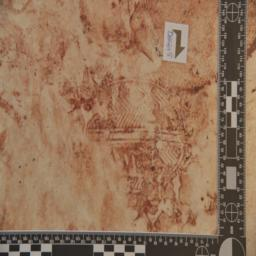
\includegraphics[width=0.5\textwidth]{data/1- Modèle Traces passives/3- Bois/Bois NH/Retouches/3.JPG}
        \caption{Sample image from the dataset}
    \end{figure}
\end{frame}

\begin{frame}
\frametitle{Dataset Architecture}
Here, you can describe the architecture of your dataset.
\begin{itemize}
\item Root directory: \texttt{analyse\_trace\_sang/IA/1- Modèle Traces passives}
\item Subdirectories: \texttt{3- Bois}, \texttt{4- Carrelage}, etc.
\item Each subdirectory contains images for a specific category.
\end{itemize}
\end{frame}

\begin{frame}
\frametitle{Model}
Here, you can describe the model you used for this classification problem.
\begin{itemize}
\item Model name: InceptionResNet (for example)
\item Reason for choosing this model
\item Any modifications made to the model
\end{itemize}
\end{frame}

\end{document}